\chapter{Accepttest of RMS Limiter}\label{app:journal_Frequency_Response2}
The purpose of this test is verify requirement 10, 11, 12, 13, and 14 concerning the RMS limiter.

\section{Setup}
The setup of this test are depicted in \autoref{fig:AcceptFreqResponse}, where the equipment is catalogued in \autoref{tab:UsedEquipmentFreqResponse}, and described as follows:

\begin{itemize}
	\item Frequency response will be measured by a Harmonie analyzer.
	\item A noise generator will generate the following for the test. 
	\begin{itemize}
		\item Sampling frequency: 48000 Hz.
		\item Generator amplitude: 10 mV, 100 mV, 200 mV, 300 mV, 400 mV, 500 mV, 600 mV, 700mV.
		\item Pink noise from 20 Hz to 20 kHz
	\end{itemize}
	\item The samples are averaged over a period of 20 seconds
	\item The software of the system used for the test is found at CD. \path{CD://Software/SystemFinal}
\end{itemize}


\subsection*{Test Setup}
\begin{figure}[H]
\centering
\includegraphics[width=0.9\textwidth]{FreqReponseSetup.png}
\label{fig:AcceptFreqResponse}
\caption{Test setup.}
\end{figure}

\subsection*{Equipment used and AAU-no.}

\begin{table}[H]
\centering
\ra{1.3}
\begin{tabular}{S[table-format=1]ccc} \toprule
    {Item} & {Description} & {AAU-no} \\ \bottomrule 
    1      &  Harmonie  & 60923  \\ 
    2      &  Harmonie PC  & 56524  \\ 
    3      &  Sine/Noise generator type 1049  & 08233  \\  \bottomrule 
\end{tabular}
\caption{Table over equipment used in the test}
\label{tab:UsedEquipmentFreqResponse}
\end{table}
\vspace{-5mm}


\section{Procedure}
The procedure for this experiment is described as follows:
\vspace{-5mm}
\begin{enumerate}
\item Setup the noise generator with the mentioned settings.
\item Setup the Harmonie and the Harmonie PC
\item Start recording on the PC
\item When finished save the results of the test.
\end{enumerate}

\section{Data Extraction}
The raw data the system can be found at the CD, \\
\path{CD://Maalinger/Maalinger210516 - Acceptance test for Limiter}\\
There are 30 bands from 20 Hz to 20 kHz, see \autoref{tb:freqBands4}, where a magnitude is given in dB for each band. 10 different measurements have been taken for both bypass and the full system. The two bands 25 Hz and 20000 Hz has been removed from the plots because of large deviation and therefore not deemed usefull.

\begin{table}[H]
\centering
\begin{tabular}{|c|c|c|c|c|c|c|c|c|c|}
\hline
\multicolumn{10}{|c|}{Bands [Hz]}                                       \\ \hline
25   & 31.5 & 40   & 50   & 63   & 80   & 100   & 125   & 160   & 200   \\ \hline
250  & 315  & 400  & 500  & 630  & 800  & 1000  & 1250  & 1600  & 2000  \\ \hline
2500 & 3150 & 4000 & 5000 & 6300 & 8000 & 10000 & 12500 & 16000 & 20000 \\ \hline
\end{tabular}
\caption{Frequency bands.}
\label{tb:freqBands4}
\end{table}

\section{Analysis}

Plotting the RMS values of the different bands stated in \autoref{tb:freqBands4} yields the graphs in \autoref{fig:RMSlimiter}. It shows how attenuation of the lower frequencies is increased as the signal amplitude is increased.

\begin{figure}[H]
	\centering
	\tikzsetnextfilename{AcceptRMS}
	% This file was created by matlab2tikz.
%
%The latest updates can be retrieved from
%  http://www.mathworks.com/matlabcentral/fileexchange/22022-matlab2tikz-matlab2tikz
%where you can also make suggestions and rate matlab2tikz.
%
\definecolor{mycolor1}{rgb}{0.00000,0.44700,0.74100}%
\definecolor{mycolor2}{rgb}{0.85000,0.32500,0.09800}%
\definecolor{mycolor3}{rgb}{0.92900,0.69400,0.12500}%
\definecolor{mycolor4}{rgb}{0.49400,0.18400,0.55600}%
\definecolor{mycolor5}{rgb}{0.46600,0.67400,0.18800}%
\definecolor{mycolor6}{rgb}{0.30100,0.74500,0.93300}%
%
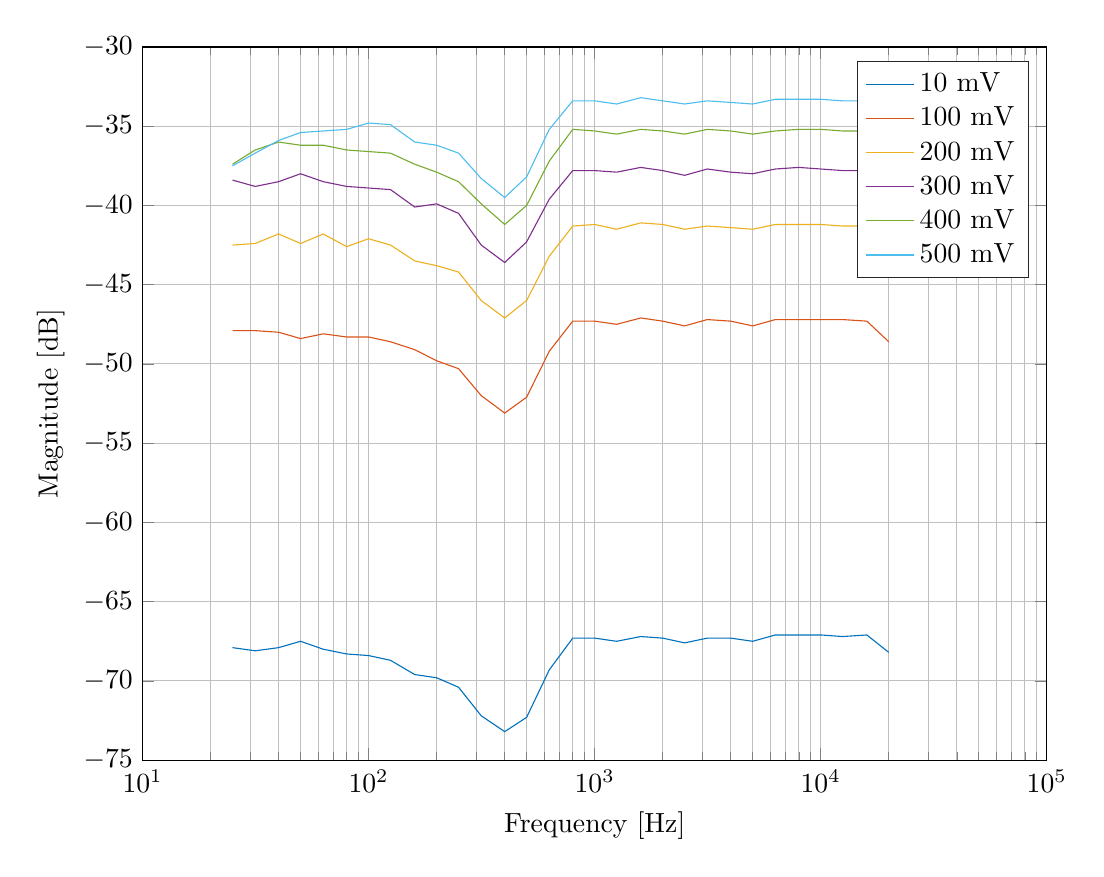
\begin{tikzpicture}

\begin{axis}[%
width=4.521in,
height=3.566in,
at={(0.758in,0.481in)},
scale only axis,
xmode=log,
xmin=10,
xmax=100000,
xminorticks=true,
xlabel={Frequency [Hz]},
xmajorgrids,
xminorgrids,
ymin=-75,
ymax=-30,
ylabel={Magnitude [dB]},
ymajorgrids,
axis background/.style={fill=white},
legend style={legend cell align=left,align=left,draw=white!15!black}
]
\addplot [color=mycolor1,solid]
  table[row sep=crcr]{%
25	-67.9\\
31.5	-68.1\\
40	-67.9\\
50	-67.5\\
63	-68\\
80	-68.3\\
100	-68.4\\
125	-68.7\\
160	-69.6\\
200	-69.8\\
250	-70.4\\
315	-72.2\\
400	-73.2\\
500	-72.3\\
630	-69.3\\
800	-67.3\\
1000	-67.3\\
1250	-67.5\\
1600	-67.2\\
2000	-67.3\\
2500	-67.6\\
3150	-67.3\\
4000	-67.3\\
5000	-67.5\\
6300	-67.1\\
8000	-67.1\\
10000	-67.1\\
12500	-67.2\\
16000	-67.1\\
20000	-68.2\\
};
\addlegendentry{10 mV};

\addplot [color=mycolor2,solid]
  table[row sep=crcr]{%
25	-47.9\\
31.5	-47.9\\
40	-48\\
50	-48.4\\
63	-48.1\\
80	-48.3\\
100	-48.3\\
125	-48.6\\
160	-49.1\\
200	-49.8\\
250	-50.3\\
315	-52\\
400	-53.1\\
500	-52.1\\
630	-49.2\\
800	-47.3\\
1000	-47.3\\
1250	-47.5\\
1600	-47.1\\
2000	-47.3\\
2500	-47.6\\
3150	-47.2\\
4000	-47.3\\
5000	-47.6\\
6300	-47.2\\
8000	-47.2\\
10000	-47.2\\
12500	-47.2\\
16000	-47.3\\
20000	-48.6\\
};
\addlegendentry{100 mV};

\addplot [color=mycolor3,solid]
  table[row sep=crcr]{%
25	-42.5\\
31.5	-42.4\\
40	-41.8\\
50	-42.4\\
63	-41.8\\
80	-42.6\\
100	-42.1\\
125	-42.5\\
160	-43.5\\
200	-43.8\\
250	-44.2\\
315	-46\\
400	-47.1\\
500	-46\\
630	-43.2\\
800	-41.3\\
1000	-41.2\\
1250	-41.5\\
1600	-41.1\\
2000	-41.2\\
2500	-41.5\\
3150	-41.3\\
4000	-41.4\\
5000	-41.5\\
6300	-41.2\\
8000	-41.2\\
10000	-41.2\\
12500	-41.3\\
16000	-41.3\\
20000	-42.5\\
};
\addlegendentry{200 mV};

\addplot [color=mycolor4,solid]
  table[row sep=crcr]{%
25	-38.4\\
31.5	-38.8\\
40	-38.5\\
50	-38\\
63	-38.5\\
80	-38.8\\
100	-38.9\\
125	-39\\
160	-40.1\\
200	-39.9\\
250	-40.5\\
315	-42.5\\
400	-43.6\\
500	-42.3\\
630	-39.6\\
800	-37.8\\
1000	-37.8\\
1250	-37.9\\
1600	-37.6\\
2000	-37.8\\
2500	-38.1\\
3150	-37.7\\
4000	-37.9\\
5000	-38\\
6300	-37.7\\
8000	-37.6\\
10000	-37.7\\
12500	-37.8\\
16000	-37.8\\
20000	-39\\
};
\addlegendentry{300 mV};

\addplot [color=mycolor5,solid]
  table[row sep=crcr]{%
25	-37.4\\
31.5	-36.5\\
40	-36\\
50	-36.2\\
63	-36.2\\
80	-36.5\\
100	-36.6\\
125	-36.7\\
160	-37.4\\
200	-37.9\\
250	-38.5\\
315	-39.9\\
400	-41.2\\
500	-40\\
630	-37.2\\
800	-35.2\\
1000	-35.3\\
1250	-35.5\\
1600	-35.2\\
2000	-35.3\\
2500	-35.5\\
3150	-35.2\\
4000	-35.3\\
5000	-35.5\\
6300	-35.3\\
8000	-35.2\\
10000	-35.2\\
12500	-35.3\\
16000	-35.3\\
20000	-36.5\\
};
\addlegendentry{400 mV};

\addplot [color=mycolor6,solid]
  table[row sep=crcr]{%
25	-37.5\\
31.5	-36.7\\
40	-35.9\\
50	-35.4\\
63	-35.3\\
80	-35.2\\
100	-34.8\\
125	-34.9\\
160	-36\\
200	-36.2\\
250	-36.7\\
315	-38.3\\
400	-39.5\\
500	-38.2\\
630	-35.2\\
800	-33.4\\
1000	-33.4\\
1250	-33.6\\
1600	-33.2\\
2000	-33.4\\
2500	-33.6\\
3150	-33.4\\
4000	-33.5\\
5000	-33.6\\
6300	-33.3\\
8000	-33.3\\
10000	-33.3\\
12500	-33.4\\
16000	-33.4\\
20000	-34.7\\
};
\addlegendentry{500 mV};

\end{axis}
\end{tikzpicture}%
	\caption{RMS limiter frequency response at different levels}
	\label{fig:RMSlimiter}
\end{figure}


\section{Error sources}

Due to large deviations in the 25 Hz and 20 kHz region, the measurements for these bands have been discarded. However since the IEC 581-6 demands only and effective frequency spectrum of 40 Hz to 16 kHz, the measurements are still deemed valid.

\section{Conclusion}

From \autoref{fig:RMSlimiter} it is hard to conclude whether the RMS limiter works or not. Under the development of the RMS limiter, the RMS limiter showed good results when lower thresholds where used. By using lower thresholds the system where able to keep the RMS value below 500 Hz under the threshold. In the acceptance test where the threshold was changed to the calculated threshold, it seen like RMS limiter is never activated. 


 showed that the RMS limiter works as es can be concluded that the RMS limiter does not attenuate as intended.

%From the test it can be concluded that the RMS limiter does not functions as expected. The gain values for the lowest frequencies are not correct since they are not attenuated equally. A not is created in the begin which can not be accounted for. There is however a slight attenuation of the lower frequencies present.  